\documentclass[a4paper,12pt]{article}
\usepackage[italian]{babel}
\usepackage[utf8]{inputenc}
\usepackage{setspace}

% Larger borders -- we do not want do waste paper, even if it is only paper on screen =)
\usepackage[top=2cm, bottom=2cm, left=2cm, right=2cm]{geometry}
% Remove auto indentation of paragraphs.
\setlength\parindent{0pt}

% Palatino font (nicer serif font: Times is for oldies)
%\renewcommand*\rmdefault{ppl}

% Nested itemize list bullet style
\renewcommand{\labelitemi}{$\bullet$}
\renewcommand{\labelitemii}{$\circ$}
\renewcommand{\labelitemiii}{--}

% Math packages
\usepackage{mathtools}
\usepackage{amsmath}
\usepackage{amsfonts}
\usepackage{amssymb}

% Graphic packages
\usepackage{graphicx}
\usepackage{subcaption}
\usepackage{float}
\usepackage{adjustbox}
\usepackage{tikz}
\usepackage{forest,array}
\usetikzlibrary{shadows}


% Graphs styles
\forestset{
  giombatree/.style={
    for tree={
      grow = east,
      parent anchor=east,
      child anchor=west,
      edge={rounded corners=2mm},
      fill=violet!5,
      drop shadow,
      l sep=10mm,
      edge path={
        \noexpand\path [draw, \forestoption{edge}] (!u.parent anchor) -- +(5mm,0) -- (.child anchor)\forestoption{edge label};
      }
    }
  }
}
\forestset{
  qtree/.style={
    for tree={
      parent anchor=south,
      child anchor=north,
      align=center,
      edge={rounded corners=2mm},
      fill=violet!5,
      drop shadow,
      l sep=10mm,
    }
  }
}

\newcommand{\projectname}{CDMA Receiver}
\newcommand{\projectnameabbr}{CDMA Rec}

% Hides ugly links from the index
\usepackage[hidelinks]{hyperref}
% Landscape format pdf pagess
\usepackage{pdflscape}

\begin{document}
\pagenumbering{gobble}

{\setstretch{1.0}
  \begin{titlepage}
  	\centering
  	
\includegraphics[width=6cm]{img/unipi.pdf}\par
    \vspace{1.5cm}
    {\Large Dipartimento di Ingegneria Dell'Informazione \par}
  	\vspace{1.5cm}
  	{\huge\textsc{\projectname{}}\par}
    \vspace{0.5cm}
    {\Large Progetto di Electronics and Comminications Systems \par}
  	\vspace{2cm}
  	Amedeo \textsc{Pochiero}\par

  	\vfill

    % Bottom of the page
  	{\large A.Y. 2019-2020\par}
  \end{titlepage}
}


\clearpage
\tableofcontents
\clearpage
\pagenumbering{arabic}

\section{Introduzione} 
  \subsection{Descrizione del Problema}
  Il collegamento broadcast può avere più nodi trasmittenti e riceventi connessi allo stesso canale broadcast condiviso. 
  In uno scenario del genere si pone il problema di come coordinare l'accesso di più nodi trasmittenti e riceventi in un
  canale broadcast condiviso, ossia il problema dell'accesso multiplo. Dato che tutti i nodi sono in grado di trasmettere
  frame, è possibile che due o più lo facciano nello stesso istante, per cui tutti i nodi riceveranno contemporaneamente
  più frame. Tra questi si genera una collisione a causa della quale nessuno dei nodi riceventi riuscirà a interpretare
  i frame.
  \subsection{CDMA}
    Il protocollo \textbf{CDMA} ( \textit{code division multiple access} ) è un protocollo a suddivisione del canale in 
    cui i vari utenti possono trasmettere contemporaneamente, causando quindi collisioni e interferenze tra loro, tuttavia
    il ricevente è in grado comunque di ricostruire il segnale trasmesso. 

    A tale scopo, ogni utente modula il proprio segnale di periodo $T_b$ ( \textit{symbol period} ) con un codice, unico
    per ogni utente, di periodo $T_c$ ( \textit{chip period} ) dove $T_c \ll T_b$ come si può vedere in Figura \ref{fig:Signals}.
    \begin{figure}[H]
      \centering
      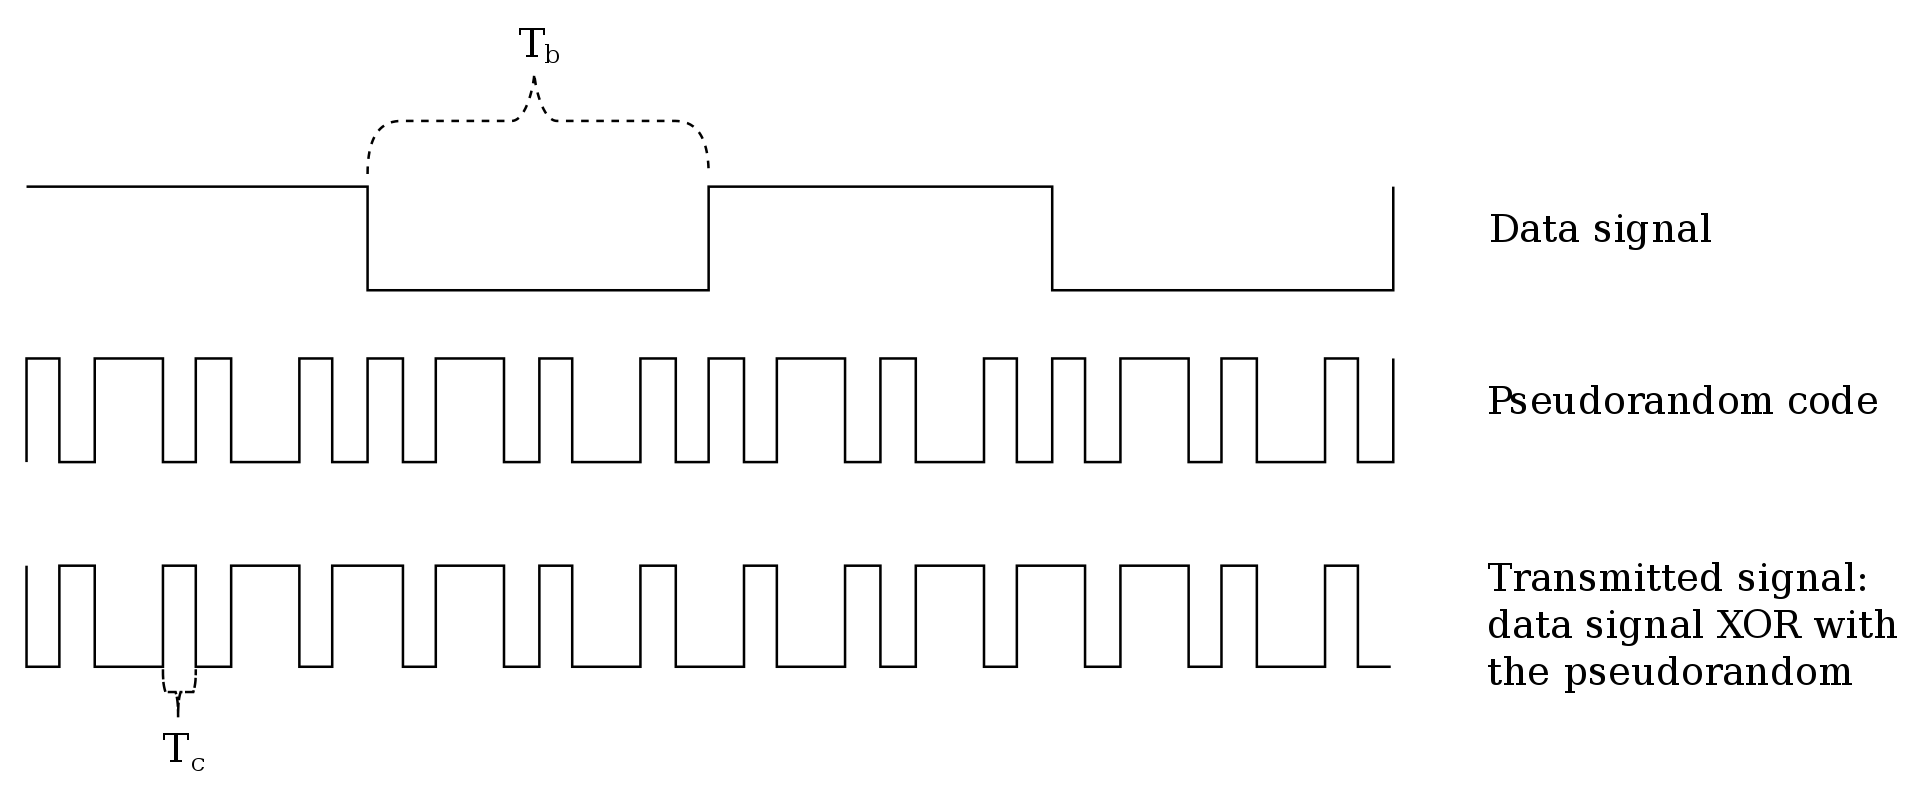
\includegraphics[width=\textwidth]{img/Generation_of_CDMA.svg.png}
      \caption{Generazione del segnale CDMA trasmesso }
      \label{fig:Signals}
    \end{figure}

    Il rapporto tra i due periodi è definito come \textit{ Spreading Factor } e come requisito è stato posto a 16:
    $$ \frac{T_b}{T_c} = 16 $$

    I codici devono essere scelti in modo tale che la correlazione tra i vari segnali dei diversi utenti sia il più vicino
    possibile a zero. Nel synchronous CDMA si può sfruttare la proprietà matematica di \textit{ortogonalità} tra vettori 
    che rappresentano stringhe di dati. Due vettori $a$ e $b$ si dicono ortogonali  se vale la seguente relazione:
    $$ a \cdot b = 0 $$

    Ogni utente deve usare un codice ortogonale a quello di tutti gli altri. Nella tabella di seguito viene riportato
    un esempio di vettori $cw_1, cw_2 \in \mathbb{Z}^{16} $  ortogonali tra di loro, i bit $0, 1$ vengono rappresentati 
    rispettivamente dai simboli $-1, 1$:

    \begin{table}[H]
      \centering
      \begin{tabular}{| c | c | c | c | c | c | c | c | c | c | c | c | c | c | c | c | c | c |}\hline
        vector & \multicolumn{16}{|c|}{bit} & Prodotto Scalare \\ \hline
        \textbf{$cw_1$} &1&1&-1&1&-1&-1&-1&1&1&-1&-1&-1&1&1&-1&1& - \\ \hline
        \textbf{$cw_2$} &1&-1&1&-1&1&-1&-1&-1&1&1&-1&-1&-1&1&-1&-1& -\\ \hline
        \textbf{$cw_{1,i} * cw_{2,i}$} &1&-1&1&-1&1&-1&-1&-1&1&1&-1&-1&-1&1&-1&-1& 0 \\ \hline
      \end{tabular}
      \caption{Vettori Ortogonali}
      \label{tab:orthogonal vectors}
    \end{table}

    \subsection{Applicazioni}
     Il \textbf{CDMA} è il protocollo di accesso a canale condiviso più diffuso nelle reti wireless e nelle tecnologie
     cellulari. Deriva da una tecnologia usata per implementare il \textbf{GPS} (\textit{Global Position System}) ed è 
     stato usato in :
     \begin{itemize}
      \item \textit{Globastar network}, con il nome di CDMA2000, ed altre compagnie telefoniche
      \item \textit{UMTS 3G} come protocollo di accesso multiplo standard
      \item \textit{OmniTRACS satellite system}, per trasporti logistici.
     \end{itemize}
  \subsection{Esempio utilizzato}\label{Esempio}
    Al fine di verificare il corretto funzionamento del ricevitore, è stato seguito un caso reale di ricezione di due bit 
    in un ricevitore CDMA. Facendo riferimento ai codici ( \textit{code words} ) della tabella \ref{tab:orthogonal vectors},
    si è considerato uno scenario in cui il primo utente trasmette il simbolo $1$, mentre un secondo utente trasmette il 
    simbolo $-1$. Per le proprietà fisiche dell'interferenza, se 2 segnali interferenti sono in fase, essi si sommano e si
    crea un segnale di ampiezza doppia, altrimenti si sottraggono e creano un segnale con un'ampiezza pari alla differenza 
    delle ampiezze. Nel mondo digitale, questo comportamento può essere rappresentato dalla somma componente per componente
    dei vettori trasmessi.

    Nella seguente tabella \ref{tab:interference pattern} il simbolo trasmesso è modulato con la rispettiva \textit{code word}, ottenendo un
    \textit{chip stream} per ogni utente. Ogni chip stream trasmesso interferisce con gli altri trasmessi nello stesso 
    istante, formando l'\textit{interference pattern}, cioè il segnale realemente ricevuto dai ricevitori.

    \begin{table}[H]
      \centering
      \begin{tabular}{| c | c | c | c | c | c | c | c | c | c | c | c | c | c | c | c | c |}\hline
        \texttt{data} & \multicolumn{16}{|c|}{\texttt{value}} \\ \hline
        $d_1$ & \multicolumn{16}{|c|}{$1$} \\ \hline
        $d_2$ & \multicolumn{16}{|c|}{$-1$}\\ \hline
        $cw_{1,i} * d_1$ &1&1&-1&1&-1&-1&-1&1&1&-1&-1&-1&1&1&-1&1 \\ \hline
        $cw_{2,i} * d_2$ &-1&1&-1&1&-1&1&1&1&-1&-1&1&1&1&-1&1&1 \\ \hline
        \textit{interference pattern} &0&2&-2&2&-2&0&0&2&0&-2&0&0&2&0&0&2 \\ \hline
      \end{tabular}
      \caption{Interferenza tra trasmettitori}
      \label{tab:interference pattern}
    \end{table}

    Per ricostruire il segnale, moltiplica ogni componente dell' \textit{interference pattern} con la propria \textit{code
    word}. Il vettore $r$ ottenuto è dato in input ad un \textit{Decisore Hard A Soglia} il quale decide il bit da porre in 
    uscita. La decisione è presa nel seguente modo:

    \begin{itemize}
      \item se $\sum\limits_{i=1}^{16} r_i \geq 0 $ allora \textit{bitstream} $= 1$
      \item se $\sum\limits_{i=1}^{16} r_i < 0 $ allora \textit{bitstream} $= 0$
    \end{itemize}

    Nell'esempio considerato i ricevitori effetturanno le seguenti operazioni:

    \begin{figure}[H]
      \centering
      \begin{tabular}{| c | c | c | c | c | c | c | c | c | c | c | c | c | c | c | c | c | c | c |}\hline
        \texttt{data} & \multicolumn{16}{|c|}{\texttt{value}} & Somma & Bit deciso\\ \hline
        $r_i * cw_{1,i}$ &0&2&2&2&2&0&0&2&0&2&0&0&2&0&0&2&16&1 \\ \hline
        $r_i * cw_{2,i}$ &0&-2&-2&-2&-2&0&0&-2&0&-2&0&0&-2&0&0&-2&-16&0 \\ \hline
      \end{tabular}
      \label{tab:Decisore}
    \end{figure}

    Come si nota dalla tabella, i ricevitori sono in grado di ricostruire il bit trasmesso originariamente ( primo utente
     $1$, secondo utente $0$) come specificato in \ref{Esempio} .


\section{Architettura}
  \subsection{Diagramma a Blocchi}
  \subsection{Implementazione}
  \subsection{Test-plan}
\section{Sintesi} 
  \subsection{Utilizzo}
  \subsection{Massima frequenza di utilizzo}
  \subsection{Cammino Critico}
  \subsection{Consumo di Potenza}
  \subsection{Warnings}
\section{Conclusioni}
\end{document}
